\documentclass[11pt]{report}
% Same style as 1-foundations/theory/preamble.tex (the course's own documents).

\usepackage[a4paper,margin=2.3cm,headheight=14pt]{geometry}
\usepackage[T1]{fontenc}
\usepackage[utf8]{inputenc}
\usepackage{lmodern}
\usepackage{microtype}
\usepackage{booktabs}
\usepackage{longtable}
\usepackage{array}
\usepackage{xcolor}
\usepackage{enumitem}
\usepackage{amssymb}
\usepackage{amsmath}
\usepackage{fancyhdr}
\usepackage{listings}
\usepackage{tikz}
\usetikzlibrary{arrows.meta,positioning,calc,fit,shapes.geometric,decorations.pathreplacing}
\usepackage[hidelinks]{hyperref}

\definecolor{warnbg}{RGB}{255,247,230}
\definecolor{warnrule}{RGB}{204,136,0}
\definecolor{newbg}{RGB}{235,245,255}
\definecolor{newrule}{RGB}{40,110,190}
\definecolor{keybg}{RGB}{237,247,237}
\definecolor{keyrule}{RGB}{50,120,60}
\definecolor{headgray}{RGB}{90,90,90}
\definecolor{codebg}{RGB}{248,248,248}

\usepackage[most]{tcolorbox}

\newtcolorbox{warnbox}[1][]{colback=warnbg,colframe=warnrule,boxrule=0.8pt,
  left=6pt,right=6pt,top=5pt,bottom=5pt,arc=1pt,#1}
\newtcolorbox{infobox}[1][]{colback=newbg,colframe=newrule,boxrule=0.8pt,
  left=6pt,right=6pt,top=5pt,bottom=5pt,arc=1pt,#1}
% "In SWEB": where the idea shows up in the course's kernel
\newtcolorbox{swebbox}[1][]{colback=newbg,colframe=newrule,boxrule=0.8pt,
  left=6pt,right=6pt,top=5pt,bottom=5pt,arc=1pt,
  title={In SWEB},fonttitle=\bfseries\small,coltitle=white,colbacktitle=newrule,#1}
% end-of-chapter summary
\newtcolorbox{keybox}[1][]{colback=keybg,colframe=keyrule,boxrule=0.8pt,
  left=6pt,right=6pt,top=5pt,bottom=5pt,arc=1pt,
  title={Key points},fonttitle=\bfseries\small,coltitle=white,colbacktitle=keyrule,#1}

\newcommand{\tbd}{\textcolor{warnrule}{\textbf{[confirm]}}}
\newcommand{\code}[1]{\texttt{#1}}
\newcommand{\file}[1]{\texttt{\small #1}}
\newcommand{\module}[1]{\textsf{module~#1}}

\setlist[itemize]{topsep=2pt,itemsep=1.5pt,parsep=0pt,leftmargin=1.3em}
\setlist[enumerate]{topsep=2pt,itemsep=1.5pt,parsep=0pt,leftmargin=1.6em}
\setlist[description]{topsep=2pt,itemsep=1.5pt,parsep=0pt,leftmargin=1.3em}

\newcolumntype{L}[1]{>{\raggedright\arraybackslash}p{#1}}

\lstset{
  language=C,
  basicstyle=\ttfamily\small,
  keywordstyle=\color{newrule}\bfseries,
  commentstyle=\color{headgray}\itshape,
  stringstyle=\color{warnrule!80!black},
  backgroundcolor=\color{codebg},
  frame=single, rulecolor=\color{black!15}, framesep=3pt,
  xleftmargin=4pt, xrightmargin=4pt, aboveskip=6pt, belowskip=4pt,
  columns=fullflexible, keepspaces=true, showstringspaces=false,
  upquote=true, tabsize=2,
  morekeywords={size_t,ssize_t,pid_t,pthread_t,pthread_mutex_t,pthread_cond_t,
                sem_t,uint8_t,uint32_t,uint64_t,bool,_Atomic,atomic_int,
                atomic_flag,__thread,_Noreturn,__asm__,volatile,pointer,uint64}
}
\lstdefinestyle{shell}{language=bash,morekeywords={},keywordstyle=\color{black}}
\lstdefinestyle{cpp}{language=C++}

\pagestyle{fancy}
\fancyhf{}
\renewcommand{\headrulewidth}{0.4pt}
\fancyhead[L]{\small\textcolor{headgray}{SWEB interview guide}}
\fancyhead[R]{\small\textcolor{headgray}{\leftmark}}
\fancyfoot[C]{\small\thepage}
\renewcommand{\chaptermark}[1]{\markboth{\thechapter\ \ #1}{}}
\fancypagestyle{plain}{\fancyhf{}\renewcommand{\headrulewidth}{0pt}\fancyfoot[C]{\small\thepage}}

\renewcommand{\arraystretch}{1.25}
\setlength{\parskip}{3pt}
\setlength{\parindent}{0pt}
\setlength{\emergencystretch}{3em}   % fewer overfull lines with long \code words

% guide additions
\newtcolorbox{lockbox}[1][]{colback=warnbg,colframe=warnrule,boxrule=0.8pt,
  left=6pt,right=6pt,top=5pt,bottom=5pt,arc=1pt,
  title={Locking},fonttitle=\bfseries\small,coltitle=white,colbacktitle=warnrule,#1}
\newtcolorbox{trapbox}[1][]{colback=warnbg,colframe=warnrule,boxrule=0.8pt,
  left=6pt,right=6pt,top=5pt,bottom=5pt,arc=1pt,
  title={Trap},fonttitle=\bfseries\small,coltitle=white,colbacktitle=warnrule,#1}
\lstset{morekeywords={ScopeLock,Mutex,Condition,SpinLock,ArchThreadRegisters,ArchMemoryMapping},
  breaklines=true, breakatwhitespace=true, postbreak=\mbox{\textcolor{headgray}{$\hookrightarrow$}\space}}
\renewcommand{\file}[1]{\texttt{#1}}   % inherit the size of the surrounding text (tables use \footnotesize)

\renewcommand{\thesection}{\arabic{section}}
\fancyhead[L]{\small\textcolor{headgray}{A1-10 shared page -- walkthrough}}
\fancyhead[R]{}
\newcommand{\done}[1]{\begin{keybox}[title={Done when}]#1\end{keybox}}
\setlist[description]{topsep=2pt,itemsep=2pt,parsep=0pt,leftmargin=1.3em}

\begin{document}

{\centering
  {\LARGE\bfseries A1-10 a page shared by two processes\par}
  \vspace{4pt}
  {\large the short version -- every line explained\par}
  \vspace{8pt}
}

\begin{infobox}
\textbf{Start:} \code{task start a1-10}. \textbf{Done:} \code{task test} shows \textbf{9 of 9} and no leak.
This code is tested (9 of 9 on your team's code). Type it yourself, one step at a time.\\[3pt]
\textbf{From the list of earlier years:} \emph{simple shm}. \textbf{Type S + E}: two syscalls + cleanup when a process ends.
\end{infobox}

% =====================================================================================
\section*{The task in 4 sentences}

\begin{enumerate}
  \item Normally every process has its own private memory -- no other process can see it.
  \item \code{shm\_attach(7)} in two processes puts the \textbf{same piece of RAM} into both: what one writes, the other reads.
  \item The kernel remembers, per key (1--15), \textbf{which piece of RAM} and \textbf{how many processes} use it.
  \item The RAM is only given back when \textbf{nobody} uses it any more (count = 0).
\end{enumerate}

\subsection*{The words you need}

{\small
\begin{tabular}{@{}L{3.3cm} L{12.1cm}@{}}
\toprule
\textbf{key} & the number (1--15) two processes agree on: ``I want shared page 7''\\
\textbf{physical page (ppn)} & a 4096-byte piece of real RAM, by its number\\
\textbf{virtual page (vpn)} & a 4096-byte piece of one process's addresses\\
\textbf{map / unmap} & enter / remove ``vpn $\to$ ppn'' in one process's page table\\
\textbf{free} & give the piece of RAM back to the kernel (\code{freePPN})\\
\textbf{count (refs)} & how many processes have the key attached\\
\textbf{leak} & RAM that is never given back -- the test checks for it at the end\\
\textbf{lock} & ``only one thread at a time in here'' -- needed because many processes use the table\\
\bottomrule
\end{tabular}}

% =====================================================================================
\subsection*{Picture 1 -- one piece of RAM in two processes}

\begin{center}
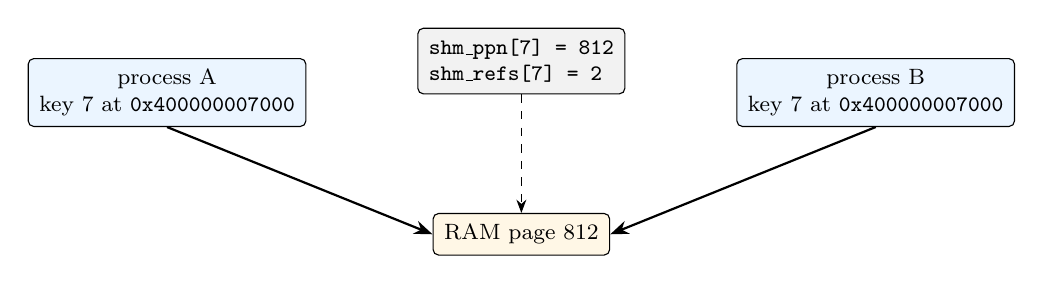
\begin{tikzpicture}[font=\footnotesize, box/.style={draw,rounded corners=2pt,align=center,inner sep=4pt}]
  \node[box,fill=newbg,minimum width=3cm] (a) at (0,0) {process A\\key 7 at \code{0x400000007000}};
  \node[box,fill=newbg,minimum width=3cm] (b) at (9,0) {process B\\key 7 at \code{0x400000007000}};
  \node[box,fill=warnbg] (p) at (4.5,-1.8) {RAM page 812};
  \node[box,fill=black!5,align=left] (t) at (4.5,0.4) {\code{shm\_ppn[7]  = 812}\\\code{shm\_refs[7] = 2}};
  \draw[-{Stealth},thick] (a.south) -- (p.west);
  \draw[-{Stealth},thick] (b.south) -- (p.east);
  \draw[dashed,-{Stealth}] (t.south) -- (p.north);
\end{tikzpicture}
\end{center}
Both page tables point to the same RAM page. Two global arrays remember it: \code{shm\_ppn} (which page)
and \code{shm\_refs} (how many users).

\subsection*{Picture 2 -- the count over time (this is exactly the test)}

\begin{center}
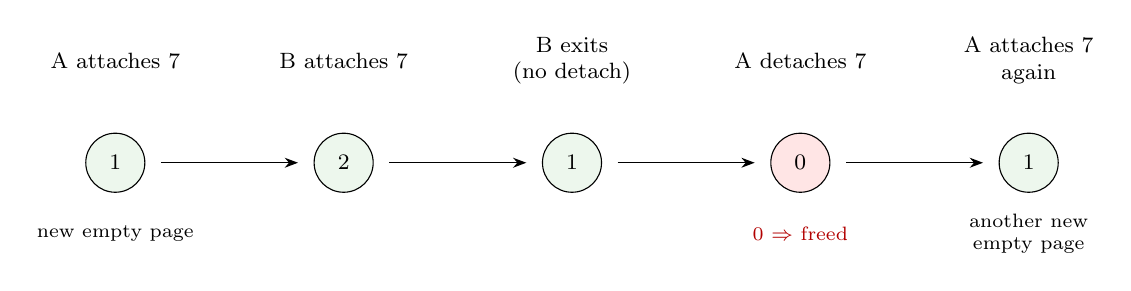
\begin{tikzpicture}[font=\footnotesize, x=2.9cm, y=1cm]
  \node[align=center] at (0,1.3) {A attaches 7};
  \node[align=center] at (1,1.3) {B attaches 7};
  \node[align=center] at (2,1.3) {B exits\\(no detach)};
  \node[align=center] at (3,1.3) {A detaches 7};
  \node[align=center] at (4,1.3) {A attaches 7\\again};
  \foreach \x/\n in {0/1,1/2,2/1,4/1} {\node[draw,circle,minimum size=0.75cm,fill=keybg] at (\x,0) {\n};}
  \node[draw,circle,minimum size=0.75cm,fill=red!10] at (3,0) {0};
  \foreach \x in {0,1,2,3} \draw[-{Stealth}] (\x+0.2,0) -- (\x+0.8,0);
  \node[align=center,font=\scriptsize] at (0,-0.9) {new empty page};
  \node[align=center,font=\scriptsize,red!70!black] at (3,-0.9) {0 $\Rightarrow$ freed};
  \node[align=center,font=\scriptsize] at (4,-0.9) {another new\\empty page};
\end{tikzpicture}
\end{center}

\subsection*{Picture 3 -- the trap: unmap must not free}

\begin{center}
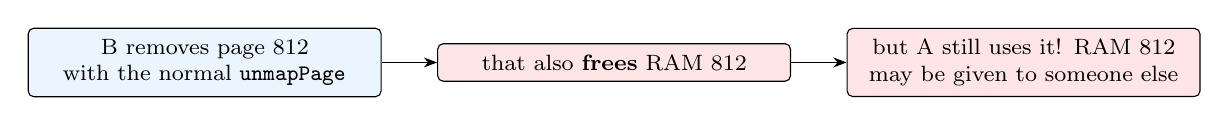
\begin{tikzpicture}[font=\footnotesize, box/.style={draw,rounded corners=2pt,align=center,inner sep=4pt,text width=4.2cm}]
  \node[box,fill=newbg] (a) at (0,0) {B removes page 812\\with the normal \code{unmapPage}};
  \node[box,fill=red!10] (b) at (5.2,0) {that also \textbf{frees} RAM 812};
  \node[box,fill=red!10] (c) at (10.4,0) {but A still uses it! RAM 812 may be given to someone else};
  \draw[-{Stealth}] (a) -- (b); \draw[-{Stealth}] (b) -- (c);
\end{tikzpicture}
\end{center}
So: a new parameter for \code{unmapPage} -- \emph{remove, but do not free} (step 2). The same trap hides in
\code{delete arch\_memory\_} at process exit: it frees \emph{every} mapped page (step 7 handles it).

\subsection*{Picture 4 -- two locks, always the same order}

\begin{center}
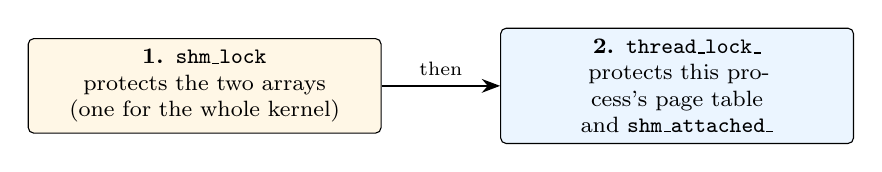
\begin{tikzpicture}[font=\footnotesize, box/.style={draw,rounded corners=2pt,align=center,inner sep=4pt}]
  \node[box,fill=warnbg,text width=4.2cm] (a) at (0,0) {\textbf{1.} \code{shm\_lock}\\protects the two arrays\\(one for the whole kernel)};
  \node[box,fill=newbg,text width=4.2cm] (b) at (6,0) {\textbf{2.} \code{thread\_lock\_}\\protects this process's page table\\and \code{shm\_attached\_}};
  \draw[-{Stealth},thick] (a) -- node[above,font=\scriptsize] {then} (b);
\end{tikzpicture}
\end{center}
A deadlock needs two threads waiting for each other's lock in \emph{opposite} order. Nothing else in the
kernel takes \code{shm\_lock}, and our code always takes it \emph{first} -- so that cannot happen.

\subsection*{Picture 5 -- where the shared pages appear}

\begin{center}
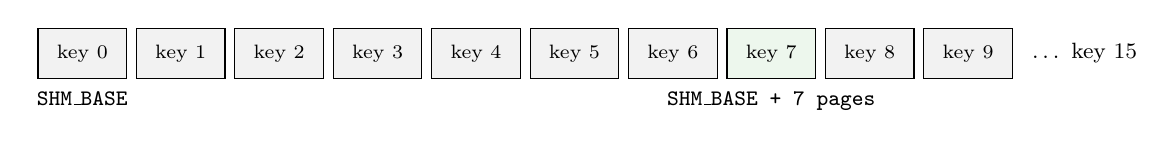
\begin{tikzpicture}[font=\footnotesize, x=1.25cm, y=0.8cm]
  \foreach \k in {0,...,9} {\draw[fill=black!5] (\k,0) rectangle +(0.9,0.8);}
  \draw[fill=keybg] (7,0) rectangle +(0.9,0.8);
  \foreach \k in {0,...,9} {\node at (\k+0.45,0.4) {\scriptsize key \k};}
  \node[right] at (10,0.4) {\ldots\ key 15};
  \node[below] at (0.45,-0.05) {\code{SHM\_BASE}};
  \node[below] at (7.45,-0.05) {\code{SHM\_BASE + 7 pages}};
\end{tikzpicture}
\end{center}
Key $k$ always appears at \code{SHM\_BASE} + $k$ pages, in every process. Key 0 is not used.

% =====================================================================================
\clearpage
\section*{The 7 steps}

{\small
\begin{tabular}{@{}l L{6.4cm} L{7.6cm}@{}}
\toprule
\# & What & File\\\midrule
1 & plumbing: numbers, libc, \code{case}s & \file{syscall-definitions.h}, \file{nonstd.h/.c}, \file{Syscall.cpp}\\
2 & unmap \emph{without} freeing & \file{ArchMemory.h/.cpp}\\
3 & constants + per-process state & \file{UserProcess.h}\\
4 & the table: 2 arrays + 1 lock & \file{UserProcess.cpp} (top), \file{main.cpp}\\
5 & attach & \file{UserProcess.cpp}\\
6 & detach & \file{UserProcess.cpp}\\
7 & cleanup when a process ends & \file{UserProcess.cpp} (destructor)\\
\bottomrule
\end{tabular}}

% =====================================================================================
\section{Plumbing}

\textbf{\file{common/include/kernel/syscall-definitions.h}} -- next to the other numbers:
\begin{lstlisting}[style=cpp,numbers=left,numberstyle=\tiny\color{headgray}]
#define sc_shm_attach 1680
#define sc_shm_detach 1681
\end{lstlisting}
\begin{description}
  \item[1--2] The numbers of the two new syscalls. The program and the kernel both include this file, so they agree.
\end{description}

\textbf{\file{userspace/libc/include/nonstd.h}} -- at the top \code{\#include "types.h"} (for \code{size\_t}); before the closing \code{\#ifdef}:
\begin{lstlisting}[style=cpp,numbers=left,numberstyle=\tiny\color{headgray}]
extern void* shm_attach(size_t key);
extern int shm_detach(size_t key);
\end{lstlisting}
\begin{description}
  \item[1] Declares \code{shm\_attach}: it gives back an address (\code{void*}).
  \item[2] Declares \code{shm\_detach}: it gives back 0 or $-1$. Without these two lines the test does not compile.
\end{description}

\textbf{\file{userspace/libc/src/nonstd.c}} -- at the end:
\begin{lstlisting}[style=cpp,numbers=left,numberstyle=\tiny\color{headgray}]
void* shm_attach(size_t key)
{
  return (void*) __syscall(sc_shm_attach, key, 0x00, 0x00, 0x00, 0x00);
}
int shm_detach(size_t key)
{
  return __syscall(sc_shm_detach, key, 0x00, 0x00, 0x00, 0x00);
}
\end{lstlisting}
\begin{description}
  \item[3] Enter the kernel with number 1680 and the key as first argument (the other four are unused).
        The result is a number -- \code{(void*)} turns it into an address; 0 becomes \code{NULL}.
  \item[7] The same with 1681. The kernel's $-1$ arrives as $-1$ in the \code{int}.
\end{description}

\textbf{\file{common/source/kernel/Syscall.cpp}} -- in the \code{switch} of \code{syscallException}, e.g.\ before \code{case sc\_execv}:
\begin{lstlisting}[style=cpp,numbers=left,numberstyle=\tiny\color{headgray}]
case sc_shm_attach:
  return_value = currentThread->getProcess()->shmAttach(arg1);
  break;
case sc_shm_detach:
  return_value = currentThread->getProcess()->shmDetach(arg1);
  break;
\end{lstlisting}
\begin{description}
  \item[1, 4] ``If the program asked for 1680 / 1681 \ldots''
  \item[2, 5] \ldots\ call the method of the \emph{calling} process with the key (\code{arg1}). \code{return\_value}
        goes back to the program.
  \item[3, 6] End of the \code{case}.
\end{description}

\done{The test compiles (it still fails -- the methods come in step 5--6).}

% =====================================================================================
\section{Unmap without freeing}

\textbf{\file{arch/x86/64/include/ArchMemory.h}} -- change the declaration of \code{unmapPage}:
\begin{lstlisting}[style=cpp,numbers=left,numberstyle=\tiny\color{headgray}]
bool unmapPage(uint64 virtual_page, bool free_physical_page = true);
\end{lstlisting}
\begin{description}
  \item[1] A second parameter: free the RAM page or not. \code{= true} is the default, so every old call
        \code{unmapPage(vpn)} still frees, exactly as before. Only our code passes \code{false}.
\end{description}

\textbf{\file{arch/x86/64/source/ArchMemory.cpp}} -- the first line of the function and the \code{freePPN} line:
\begin{lstlisting}[style=cpp,numbers=left,numberstyle=\tiny\color{headgray}]
bool ArchMemory::unmapPage(uint64 virtual_page, bool free_physical_page)
...
  if (free_physical_page)
    PageManager::instance()->freePPN(m.page_ppn);
\end{lstlisting}
\begin{description}
  \item[1] The same parameter, without the \code{= true} (the default belongs only in the \file{.h}).
  \item[3--4] Free the RAM page only if asked to. The rest of \code{unmapPage} (remove the entry) stays as it is.
\end{description}

\done{\code{unmapPage(vpn, false)} removes the page from the page table but keeps the RAM (picture 3).}

% =====================================================================================
\section{Constants and per-process state \hfill {\normalsize\file{common/include/kernel/UserProcess.h}}}

\begin{lstlisting}[style=cpp,numbers=left,numberstyle=\tiny\color{headgray}]
#define SHM_KEYS 16
#define SHM_BASE 0x0000400000000000ULL

size_t shmAttach(size_t key);
size_t shmDetach(size_t key);

bool shm_attached_[SHM_KEYS] = {};
\end{lstlisting}
\begin{description}
  \item[1] \emph{(at the top, next to the other \code{\#define}s)} 16 slots: keys 1--15, slot 0 unused.
  \item[2] The address of ``key 0''; key $k$ is $k$ pages above it (picture 5). Far away from code, heap and stacks.
  \item[4--5] \emph{(in the \code{public:} part, e.g.\ after \code{cancelThread})} The two methods the \code{case}s
        call. Public, so \file{Syscall.cpp} may call them.
  \item[7] \emph{(in the \code{private:} part, at the bottom)} One flag per key: ``\emph{this} process has it mapped''.
        \code{= \{\}} starts all as \code{false}. Needed to answer: attach twice? detach without attach? what to
        clean up at exit?
\end{description}

\done{The constants, two declarations and one member are in \file{UserProcess.h}.}

% =====================================================================================
\section{The table: two arrays and one lock}

\textbf{\file{common/source/kernel/UserProcess.cpp}} -- below the \code{\#include}s (add \code{\#include "ScopeLock.h"}):
\begin{lstlisting}[style=cpp,numbers=left,numberstyle=\tiny\color{headgray}]
size_t shm_ppn[SHM_KEYS] = {};
size_t shm_refs[SHM_KEYS] = {};
Mutex* shm_lock = nullptr;
\end{lstlisting}
\begin{description}
  \item[1] Per key: which RAM page belongs to it. 0 = no page yet.
  \item[2] Per key: how many processes have it attached.
  \item[3] The lock for both arrays (picture 4). Only a \emph{pointer}: SWEB never runs constructors of global
        objects, and a \code{Mutex} needs its constructor. Plain number arrays need none -- they are just 0.
  \item[1--3] They are outside any class: one table for the whole kernel, shared by all processes.
\end{description}

\textbf{\file{common/source/kernel/main.cpp}} -- \code{\#include "Mutex.h"} at the top, then:
\begin{lstlisting}[style=cpp,numbers=left,numberstyle=\tiny\color{headgray}]
extern Mutex* shm_lock;

  shm_lock = new Mutex("shm_lock");
\end{lstlisting}
\begin{description}
  \item[1] \emph{(at file level, above \code{startup()})} ``This variable exists in another file'' -- so
        \file{main.cpp} may use it.
  \item[3] \emph{(in \code{startup()}, right after \code{Scheduler::instance();})} Create the lock once at boot,
        before any program can attach.
\end{description}

\done{It compiles except for the two missing methods.}

% =====================================================================================
\section{Attach \hfill {\normalsize\file{UserProcess.cpp}, at the end}}

\begin{lstlisting}[style=cpp,numbers=left,numberstyle=\tiny\color{headgray}]
size_t UserProcess::shmAttach(size_t key)
{
  if (key == 0 || key >= SHM_KEYS)
    return 0;
  size_t vpn = SHM_BASE / PAGE_SIZE + key;
  ScopeLock global(*shm_lock);
  ScopeLock local(thread_lock_);
  if (!shm_attached_[key])
  {
    if (shm_refs[key] == 0)
      shm_ppn[key] = PageManager::instance()->allocPPN();
    shm_refs[key]++;
    bool mapped = arch_memory_->mapPage(vpn, shm_ppn[key], 1);
    assert(mapped);
    shm_attached_[key] = true;
  }
  return vpn * PAGE_SIZE;
}
\end{lstlisting}
\begin{description}
  \item[3--4] Only keys 1--15 exist. Otherwise return 0 = \code{NULL} (the test tries 0 and 16).
  \item[5] The key's fixed virtual page number: \code{SHM\_BASE} as a page number, plus the key (picture 5).
  \item[6] Take the table lock first \ldots
  \item[7] \ldots\ then this process's lock. Same order everywhere (picture 4). Both are released
        automatically at every \code{return}.
  \item[8] Only if this process does not have the key yet -- attaching twice must not map twice or count twice.
  \item[10--11] Nobody uses the key yet: take a fresh piece of RAM. \code{allocPPN} fills it with zeros
        (``the first attach creates the page, zeroed'').
  \item[12] One more user.
  \item[13] Enter ``vpn $\to$ RAM page'' in \emph{this} process's page table; \code{1} = the program may access it.
        \code{mapPage} returns \code{false} only if the vpn is already mapped \ldots
  \item[14] \ldots\ which cannot happen (line 8 checked it) -- the \code{assert} would catch a bug.
        (\code{mapPage} is \code{[[nodiscard]]}: its result must be used.)
  \item[15] Remember: this process has the key now.
  \item[17] The address = page number $\times$ 4096. Also for the second attach: the same address.
\end{description}

\done{Attach maps the page once per process and counts each process once.}

% =====================================================================================
\section{Detach \hfill {\normalsize\file{UserProcess.cpp}}}

\begin{lstlisting}[style=cpp,numbers=left,numberstyle=\tiny\color{headgray}]
size_t UserProcess::shmDetach(size_t key)
{
  if (key == 0 || key >= SHM_KEYS)
    return (size_t) -1;
  ScopeLock global(*shm_lock);
  ScopeLock local(thread_lock_);
  if (!shm_attached_[key])
    return (size_t) -1;
  arch_memory_->unmapPage(SHM_BASE / PAGE_SIZE + key, false);
  ArchMemory::flushTlb();
  shm_attached_[key] = false;
  shm_refs[key]--;
  if (shm_refs[key] == 0)
    PageManager::instance()->freePPN(shm_ppn[key]);
  return 0;
}
\end{lstlisting}
\begin{description}
  \item[3--4] Invalid key $\to$ $-1$.
  \item[5--6] The two locks, same order as in attach.
  \item[7--8] Not attached in this process $\to$ $-1$ (``detaching twice fails'').
  \item[9] Remove the page from this process's page table, \textbf{\code{false} = keep the RAM} -- others may use it.
  \item[10] The CPU caches translations (TLB). Flush, so it forgets the old one and a later access really fails.
  \item[11] This process no longer has the key.
  \item[12] One user less.
  \item[13--14] Nobody left: now give the RAM back (``after the last detach the page was freed'').
        \code{shm\_ppn[key]} keeps the old number, but \code{shm\_refs} is 0 -- the next attach takes a new page (line 10 of attach).
  \item[15] Success.
\end{description}

\done{Detach removes the page and frees the RAM only for the last user.}

% =====================================================================================
\section{Cleanup when a process ends \hfill {\normalsize\file{UserProcess.cpp}, \textasciitilde UserProcess}}

Between \code{delete loader\_;} and \code{delete arch\_memory\_;}:
\begin{lstlisting}[style=cpp,numbers=left,numberstyle=\tiny\color{headgray}]
{
  ScopeLock global(*shm_lock);
  for (size_t key = 1; key < SHM_KEYS; ++key)
  {
    if (!shm_attached_[key])
      continue;
    arch_memory_->unmapPage(SHM_BASE / PAGE_SIZE + key, false);
    shm_refs[key]--;
    if (shm_refs[key] == 0)
      PageManager::instance()->freePPN(shm_ppn[key]);
  }
}
\end{lstlisting}
\begin{description}
  \item[Why at all] A program may end \emph{without} \code{shm\_detach} (the test's second child does).
        Then \code{delete arch\_memory\_} would free every mapped page -- also the shared one (picture 3).
  \item[1, 12] An extra block: the lock of line 2 is released at line 12, before \code{delete arch\_memory\_}.
  \item[2] The table lock (we change \code{shm\_refs}). No \code{thread\_lock\_}: the process is being deleted,
        none of its threads runs any more.
  \item[3] Go through all keys 1--15.
  \item[5--6] Skip the keys this process does not have.
  \item[7] Remove the page, keep the RAM -- \emph{before} \code{delete arch\_memory\_} could free it.
  \item[8--10] One user less; free the RAM if it was the last (otherwise: a leak at the end of the test).
\end{description}

\done{\code{task test}: \textbf{9 of 9 passed}, \code{sweb\_run status 0} (no leak).}

% =====================================================================================
\section*{The test -- what each check means}

{\small
\begin{tabular}{@{}L{6.8cm} L{8.4cm}@{}}
\toprule
\textbf{Check} & \textbf{Made to pass by}\\\midrule
attached key 7 & steps 1--5\\
attaching twice gives the same address & attach, line 8 + 17\\
child sees the parent's text / wrote into our page & one RAM page in two page tables (picture 1)\\
page survives a child that did not detach & step 7 + \code{false} in step 2: count 2 $\to$ 1, RAM kept\\
detached & step 6\\
detaching twice fails & detach, lines 7--8\\
after the last detach the page was freed: a new one is zero & detach lines 13--14, then attach lines 10--11\\
invalid keys rejected & attach, lines 3--4\\
no leak at the end & step 7: the parent ends attached, its count is dropped and the RAM freed\\
\bottomrule
\end{tabular}}

\section*{Remember -- and the tutor questions}

\begin{keybox}[title={Three sentences}]
\begin{enumerate}
  \item One RAM page in several page tables; two arrays remember the page and \textbf{count the users} per key.
  \item Removing a shared page \textbf{never frees} it -- only the last user (count 0) frees it, also at process exit.
  \item Two locks, \textbf{always \code{shm\_lock} first}, then \code{thread\_lock\_} -- that rules out a deadlock.
\end{enumerate}
\end{keybox}

{\small
\begin{tabular}{@{}L{6.2cm} L{9.0cm}@{}}
\toprule
\textbf{Question} & \textbf{Short answer}\\\midrule
How do two processes see the same memory? & both page tables point to the same RAM page\\
Why count the users? & the RAM may only be freed when the last one is gone\\
Why not the normal \code{unmapPage}? & it frees the RAM, the other process would lose its page\\
A process exits without detaching? & the destructor unmaps without freeing and lowers the count\\
Why is the lock created in \code{startup()}? & SWEB does not run constructors of global objects\\
Why can't the two locks deadlock? & same order everywhere, and nothing else takes \code{shm\_lock}\\
Why \code{flushTlb} in detach? & the CPU might still use the old translation\\
What would \code{fork} do with an attached page? & your team's fork copies the address space: the child gets a private copy, not the shared page\\
\bottomrule
\end{tabular}}

\end{document}
